\documentclass[12pt,a4paper, twoside]{report}
\usepackage[utf8]{inputenc}
\usepackage[english]{babel}
\usepackage{amsmath}
\usepackage{amsfonts}
\usepackage{amssymb}
\usepackage{graphicx}
\usepackage{lmodern}

% For hyperlinks and meta data
\usepackage{hyperref}
\hypersetup{
    bookmarks=true,         % show bookmarks bar?
    unicode=false,          % non-Latin characters in Acrobat’s bookmarks
    pdftoolbar=true,        % show Acrobat’s toolbar?
    pdfmenubar=true,        % show Acrobat’s menu?
    pdffitwindow=false,     % window fit to page when opened
    pdfstartview={FitH},    % fits the width of the page to the window
    pdftitle={Simulation of complex actuators},    % title
    pdfauthor={Hubert Woszczyk},     % author
    pdfsubject={Master thesis},   % subject of the document
    pdfcreator={TexMaker},   % creator of the document
    pdfproducer={ULg}, % producer of the document
    pdfkeywords={robotics, physics, bullet, blender}, % list of keywords
    pdfnewwindow=true,      % links in new PDF window
    colorlinks=true,       % false: boxed links; true: colored links
	linktocpage=true,    
    linkcolor=red,          % color of internal links (change box color with linkbordercolor)
    citecolor=blue,        % color of links to bibliography
    filecolor=magenta,      % color of file links
    urlcolor=cyan           % color of external links
}
% Margins
\usepackage[left=2cm,right=2cm,top=2cm,bottom=2cm]{geometry}

% For nice tables
\usepackage{booktabs,tabularx}
\usepackage[tableposition=top]{caption}
\captionsetup[table]{singlelinecheck=off}

\usepackage{cleveref} %should be the last package

\begin{document}

\begin{titlepage}


\begin{center}
\large
University of Liège - Faculty of engineering
\end{center}

\vfill

\begin{minipage}{0.5\textwidth}

\includegraphics[width=0.9\textwidth]{figures/ULg_logo_couleur.pdf}
\end{minipage}
\begin{minipage}{0.5\textwidth}
\huge
\textbf{Master thesis}\\\\
\normalsize
\textbf{Simulation of complex actuators}\\\\
Author : Hubert Woszczyk\\
Promotor : Pr. Bernard Boigelot\\
\end{minipage}

\vfill
\begin{center}
\large
Master thesis conducted for obtaining the\\ Master's degree in Electrical Engineering\\ by Hubert Woszczyk\\
\vspace*{8cm}
\normalsize
Academic year 2015-2016
\end{center}

\end{titlepage}

\newpage\null\thispagestyle{empty}\newpage

\thispagestyle{empty}
\begin{center}
    \Large
    \textbf{Simulation of complex actuators}
    
    \vspace{0.4cm}
    \large
    Hubert Woszczyk, under the supervision of Pr. Bernard Boigelot
    
    \normalsize
    Academic year 2015-2016\\
    Faculty of Applied Sciences\\
    Electrical Engineering
    
    \vspace{0.9cm}
    \textbf{Abstract}
\end{center}
The word \emph{robot} has been crafted by Czech writer Karel Čapek in his play R.U.R. (Rossum's Universal Robots) in the beginning of the XXth century and is derived from the slavic world \emph{robota} which means \emph{labour} or \emph{work}.


\clearpage
\pagenumbering{roman}
\setcounter{page}{1}
\chapter*{Acknowledgements}
My first thanks go to Prof. Bernard Boigelot who made it possible for numerous students, including me, to work in the passionate field of robotics. I also wish to thank him for his guidance, help and accessibility.

I am deeply grateful to my friends Elodie and Laurine for reading and correcting this manuscript. I also want to thank fellow students Grégory Di Carlo and Guillaume Lempereur with whom I had the pleasure of working together one last time.

Finally, I would like to express my sincere thanks to all those who helped me complete this master thesis.

\thispagestyle{plain}
\begin{center}
    \Large
    \textbf{Simulation of complex actuators}
        
    \vspace{0.4cm}
    \large
    Hubert Woszczyk
    \normalsize
    
    \vspace{0.9cm}
    \textbf{Abstract}
\end{center}
Lorem ipsum dolor...



\chapter*{Acknowledgments}
I want to thank:
\begin{itemize}
\item Grégory Di Carlo, for the textures he provided me with.
\end{itemize}

\tableofcontents

\listoffigures

%% Intro
\chapter{Introduction}
\section{Introduction}
\section{Context}
For the last ten years, students from the Montefiore institute have been participating in a robotic contest named \emph{Eurobot}, a competition in which wheeled robots battle each other for points in various play environments. After some success and following a thirst for new challenges, it was decided to move on to another contest, \emph{RoboCup}.

\begin{figure}[htp]
\center
\begin{subfigure}[b]{0.45\textwidth}
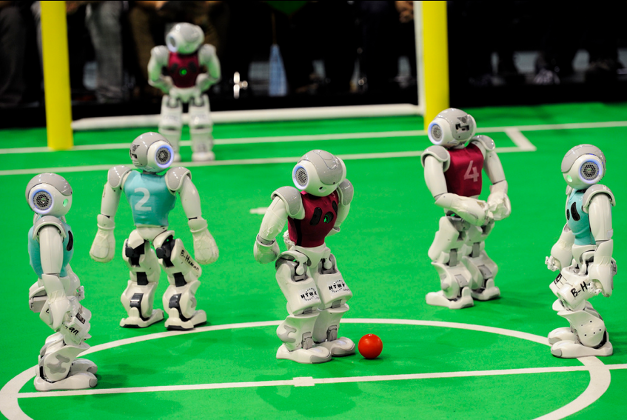
\includegraphics[width=\textwidth]{figures/intro_standard}
\caption[RoboCup Soccer standard platform]{Two teams of Nao robots playing against each other in the 2014 edition of RoboCup Soccer standard platform league. \textit{[Photo courtesy of RoboCup]}}
\label{fig:intro_standard}
\end{subfigure}
\hfill
\begin{subfigure}[b]{0.45\textwidth}
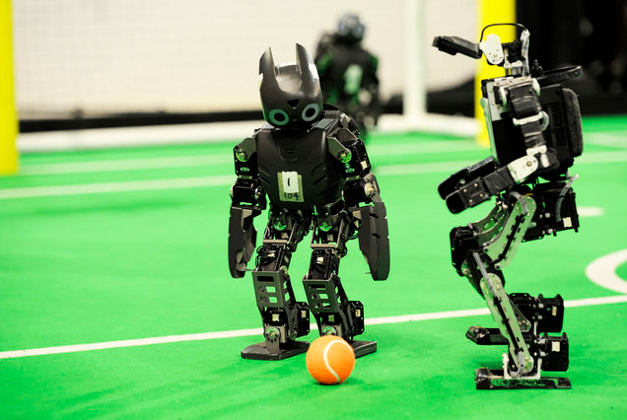
\includegraphics[width=\textwidth]{figures/intro_ks}
\caption[RoboCup Soccer standard platform]{Two robots of opposing teams looking at the ball, in the 2013 edition of RoboCup Soccer kidsize league. \textit{[Photo courtesy of RoboCup]}}
\label{fig:intro_ks}
\end{subfigure}
\caption[RoboCup standard and kidsize leagues]{Robocup standard and kidsize leagues}
\label{fig:intro_robocup}
\end{figure}

This contest is quite vast and, as of 2016, is divided into several categories (called domains in RoboCup jargon):
\begin{itemize}
\item RoboCup Rescue: as the name suggests, a domain where robots must perform various rescue operations in diverse scenarios.
\item RoboCup Industrial: a category with industrially oriented competitions.
\item RoboCup@Home: centred around domestic robots, such as robotics helpers for the elderly or robotic butlers.
\item RoboCupJunior: more of an initiative that aims to foster robotics interest in children rather than a contest, it helps organize various robotics events for younger minds.
\item RoboCup Soccer: historically the first category, centred about humanoid robots playing football. The objective of this category is to have a team of robots beat the world champions by 2050. This is the category we will compete in.
\end{itemize}

RoboCup Soccer is further subdivided into 4 sub-categories called leagues:\begin{itemize}
\item Standard platform, where the teams all use the same robot, \emph{Nao}, as illustrated in \Cref{fig:intro_standard}.
\item Simulation, a league that does not feature physical robots but focuses on team strategies and artificial intelligence. The matches take place in 2D or 3D simulators.
\item Adultsize, for the taller robots.
\item Teensize, for middle sized robots.
\item Kidsize, for the smaller robots. \Cref{fig:intro_ks} shows a match in progress from that league.
\end{itemize}

This year's team is preparing to participate to the Kidsize league and this master's thesis, along with two others, is the by-product of that team's activity. Since this is our first time participating we have no experience regarding humanoids robots. To avoid spending countless hours building and testing different designs we need a tool able of simulating a robot model and its interactions with a physical world.  

\section{Goals of the project}
The goal of this thesis is to provide the team with a physics simulating tool with the following features:
\begin{itemize}
\item realistic simulation of the physics of rigid bodies. This means that the tool should handle inertia, collisions, friction and constraints between objects. Simulation of springs and dampers is an interesting bonus.
\item receive and process orders incoming at a relatively high frequency. The processing need not be in real-time.
\item the model of our robot should receive the same orders as the real robot would. That is, the simulator should provide the same interface to the control code as the real robot would. 
\item 3D visualization of the simulation.
\end{itemize}

That simulator will be used to:
\begin{enumerate}
\item Test different robot designs and choose the best one, in a more efficient way than it could be achieved by physically building the designs.
\item Speed up development and testing of the control code because multiple teams will be able to work in parallel. 
\end{enumerate}

\section{Structure of the report}
This report begins with an overview of the basic concepts behind physics simulation on computers in \cref{chap:principles}. We then move on to \cref{chap:choice} that explains the problem we want to solve and motivates the choice of V-Rep as the main simulation tool for this project.

\Cref{chap:modelling} is about the modelling of our humanoid robot in preparation for \cref{chap:simulation} to go into the core of the subject with some simulations. \Cref{chap:simulation} also explains how our work influenced the design of the robot.

\Cref{chap:conclusion} concludes this work by summing up what is achieved and laying out future prospects.

%% Pre-work
\chapter{Setting up the simulation}

\section{Choosing the right engine}
\cite{blender_for_robotics}
The list of physics simulating engines is quite long, but the most popular ones are, in no particular order
\begin{enumerate}
\item Bullet
\item ODE
\item DART
\item Simbody
\item PhysX
\item Havok
\end{enumerate}
Bullet was chosen because while it does not distinguish itself when it comes to pure physical simulation \cite{engines_comparison}, a 3D modelling application called Blender is built atop of it, providing excellent tools for fast and easy robot modelisation. Blender also provides access to Bullet through a well document Python API.

\begin{table}[htp]
\center
\caption{Features comparison}
\begin{tabularx}{\textwidth}{@{} X X X X X X @{}}
\toprule
\textbf{Engine} & \textbf{License} & \textbf{Coordinates} & \textbf{Origin} & \textbf{Editor} &\textbf{Solver type}\\ 
\midrule
Bullet & Free & Maximal & Games & Blender & Iterative \\ 

ODE & Free & Maximal & Simplified robot dynamics, games & & Iterative\\ 

DART & Free & Generalized & Computer graphics, robot control & &\\

Simbody & Free & Generalized & Biomechamics & \\

PhysX & Proprietary & Maximal & Games & \\

Havok & Proprietary & Maximal & Games & \\
\bottomrule
\end{tabularx}
\label{table:specs}
\end{table}

\section{Settings}
To have satisfactory results some settings need to set correctly.
\begin{itemize}
\item The timestep
\item The number of solver iterations
\item The numbe of sub steps
\end{itemize}

\section{Model}
 

\chapter{Conclusion}

\bibliographystyle{plain}
\bibliography{bib} 

\end{document}